To obtain reliable models, one must both choose or create a training set
carefully and study the impact of various algorithm parameters on the error.
Although the title of this section suggests final steps of confirming a model's
usefulness for predictions, what follows is more of a diagnostic exercise. 
In practice, these analyses can be used for both purposes.

\gls{ML} algorithms are heavily dependent on the training inputs and algorithm
parameters given to them, such as training set sizes, regularization, number of
features in the training set, optimization parameters, etc.  From the results
shown in Section \ref{sec:statmodel}, it is clear there is room for
improvement.  To evaluate these input and parameter variations, diagnostic
plots show the errors between the predicted burnup values and the actual burnup
values with respect to some variable on the \textit{x}-axis.  As previously
introduced in Section \ref{sec:optvalid}, the prediction errors are compared to
the training error to understand the generalization strength. These two errors
are plotted with respect to training set size (learning curves) and the
algorithm parameters governing model complexity (validation curves) to provide
insight into the model fitness. 

In addition to \gls{ML} best practices, another layer of comparison is added
here.  Because it is difficult to ensure consistently representative testing
data, the accuracy of a learned model should not depend on only one testing
set.  The learned model's accuracy is better estimated by using a validation
set. Here, this is implemented as \textit{k}-fold \gls{CV}, introduced
in Section \ref{sec:selectass}. This work includes both the testing error
(using the testing set described in Section \ref{sec:training}) and $5$-fold
\gls{CV} error. The predetermined testing set will allow for comparison
against the previous work it was obtained from \cite{dayman_feasibility_2013},
but it is assumed that \gls{CV} will provide a better indication of
model performance because the entirety of the training set has also been
tested.  The testing error scenario performs fitting and prediction $n=10$
times and averages the errors of those results.

\begin{figure}[!htb]
    \centering
    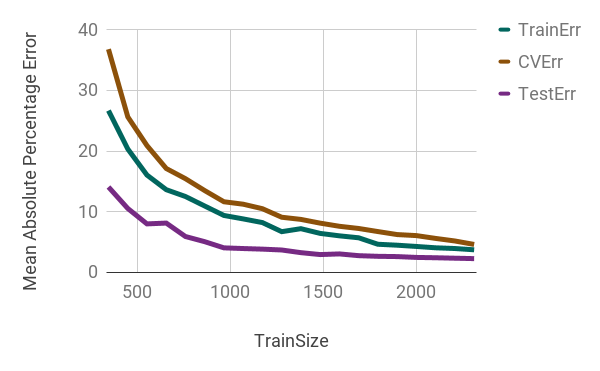
\includegraphics[width=\linewidth]{./chapters/demo_method/lc1.png}
    \caption{\acrshort{SVR} Learning Curve for Burnup Prediction, $TrainSet\ Size = 2313$}
    \label{fig:lc1}
\end{figure}

The learning curves are obtained as follows, shown in Figure \ref{fig:lc1}.
For a given (randomly chosen) training set size between $15$ and $100\%$ of the
total data set, training and prediction rounds were performed for each. 

What one seeks from a learning curve is for the training and \gls{CV}/testing
curves to approach each other, but also for the magnitude of the error to be
acceptable. As the training set size reaches $100\%$, both the training and
\gls{CV} errors do approach the training error curve.  However, the testing
error here is \textbf{lower} than the training error, and this does not happen
unless there is an issue with the training and/or testing sets. One possible
explanation is that the testing set, while the values were chosen to be between
the data points of the training set, somehow fit the model too well. This is
the danger with systematically choosing a testing set, and why the \gls{CV}
error is used. 

While the \gls{CV} error performs as expected, in that it approaches and
remains below the training error curve, but the parallel nature of the plot is
not typical. There is no example behavior of the exact shape of Figure
\ref{fig:lc1}'s learning curve in Figure \ref{fig:learning}. This could
indicate overfitting (high variance) because of the consistent gap.  More
robust diagnostics are needed to confirm the model is overfit.  It is presumed
this is not caused by the algorithms, but the training set itself.  It is
likely covering too small of a range of the simulation space.

\begin{figure}[!htb]
    \centering
    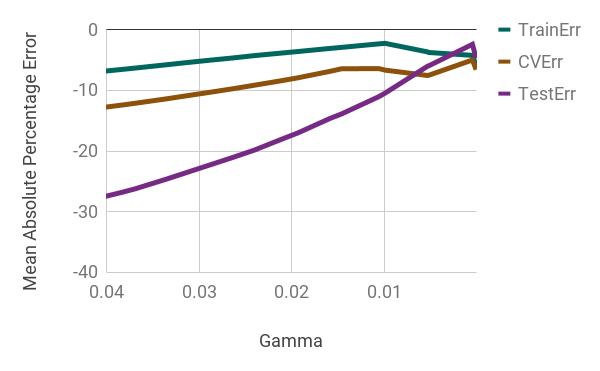
\includegraphics[width=\linewidth]{./chapters/demo_method/vc1.png}
    \caption{\acrshort{SVR} Validation Curve for Burnup Prediction, $\gamma = 0.001$}
    \label{fig:vc1}
\end{figure}

The validation curves are obtained as follows, shown in Figure \ref{fig:vc1}.
The $\gamma$ parameter in \gls{SVR} was varied from $10^{-4}-10^{-2}$.  Note
that in Figure \ref{fig:vc1} the domain has been decreased to show the features
close to the \textit{y}-axis.  Training and prediction rounds were carried out
for each value of $\gamma$ with described above.  $5$ \gls{CV} folds with $10$
prediction trials.  As with Figure \ref{fig:lc1}, the testing curve is above
the training curve, but only for small values of $\gamma$.  More work is
needed, but there is a possible \gls{CV} minimum at $\gamma=0.001$.  This was
also done for the $C$ parameter, which was varied from $10^{-2}-10^{5}$, not
pictured. The ideal $C$ in this case was $10^{3}$.  If the model is under- or
overfit, not much variation will be seen with respect to the algorithm
parameters. The resolution to the under- or overfitting is discussed in Section
\ref{sec:prep}.


